\documentclass[a4paper]{article}

\usepackage[T2A]{fontenc}
\usepackage[utf8]{inputenc}
\usepackage[russian]{babel}
\usepackage{graphicx}
\usepackage{float}
\usepackage{mathtools}
\usepackage{wrapfig}
\usepackage{amsfonts, amssymb, amsmath, latexsym}
\usepackage{nicefrac}
\usepackage{hhline}
\usepackage{multirow}
\usepackage[colorlinks=true,linkcolor=blue,citecolor=blue]{hyperref}       % hyperlinks
\usepackage{nicefrac}       % compact symbols for 1/2, etc.
\usepackage{nameref}
\usepackage{booktabs}       % professional-quality tables
\usepackage{algorithm}
\usepackage{algpseudocode}
\usepackage{xcolor, colortbl}
\usepackage{etoolbox}
\usepackage{tikz}
\usepackage{bookmark}

% \graphicspath{ {./} }

\usepackage[verbose=true,letterpaper]{geometry}

\newgeometry{
    textheight=25cm,
    textwidth=18cm,
    top=2.5cm,
    headheight=12pt,
    headsep=10pt,
    footskip=1cm,
    marginparwidth=15pt
}

%\usepackage{showframe} 

\usepackage{epigraph}
\usepackage{amsmath,amsfonts,amssymb,amsthm,mathtools, mathrsfs}
\usepackage{amsthm}

\title{Работа 4.3.1 \\ Дифракция}
\author{Шарапов Денис, Б05-005}
\date{}

\usepackage{fancyhdr}
\pagestyle{fancy}
\fancyhf{}
\rhead{Работа 4.3.1}
\lhead{}
\cfoot{\thepage}
\usepackage{subcaption}
\usepackage[font={small}]{caption}

\begin{document}

    \maketitle
    \tableofcontents
    \newpage
    
\section{Аннотация}

\noindent\textbf{Цель работы:} Исследовать явления дифракции Френеля и Фраунгофера на щели, изучить влияние дифракции на разрешающую способность оптических приборов. \smallskip
 
\noindent \textbf{В работе используются:} оптическая скамья, ртутная лампа, монохроматор, щели с регулируемой шириной, рамка с вертикальной нитью, двойная щель, микроскоп на поперечных салазках с микрометрическим винтом, зрительная труба.

\section{Результаты измерений и обработка данных}

\subsection{Дифракция Френеля на щели}

\begin{figure}[ht!]
    \centering
    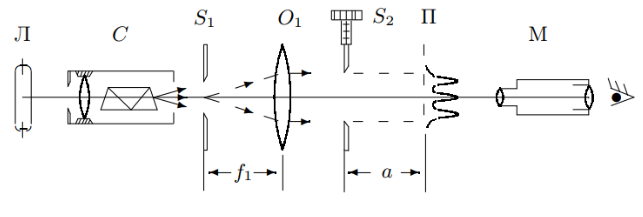
\includegraphics[width = 0.75\textwidth]{image/pic1.png}
    \caption{Схема лабораторной установки для наблюдения дифракции Френеля}
\end{figure}

\noindent Измерим ширину $b$ щели $S_2$ с помощью микрометрического винта и поперечных салазок микроскопа: $$b_{\text{микр}} = (2,740 \pm 0,005) \cdot 10^{-4} \;\; \text{м},$$ $$b_{\text{щель}} = (3,00 \pm 0,05)\cdot 10^{-4} \;\; \text{м}.$$

\noindent Зависимость координаты микроскопа от числа наблюдаемых полос представлена в таблице 1.

\begin{table}[!ht]
    \centering
    \caption{Зависимость координаты микроскопа от числа наблюдаемых полос}
    \begin{tabular}{|c|c|c|c|c|c|c|}
    \hline
    $n$, шт    & 0   & 1   & 2   & 3   & 4   & 5   \\ \hline
    $z$, мм    & 481 & 475 & 467 & 462 & 460 & 459 \\ \hline
    $a$, мм    & 28  & 22  & 14  & 9   & 7   & 6   \\ \hline
    $\xi$, мм & --- & 110 & 124 & 121 & 124 & 128 \\ \hline
    \end{tabular}
\end{table}

\noindent Построим график зависимости $\xi (n)$ ($\xi_{n} = \sqrt{an\lambda}$, $\lambda = 546,1$ нм).

\begin{figure}[ht!]
    \centering
    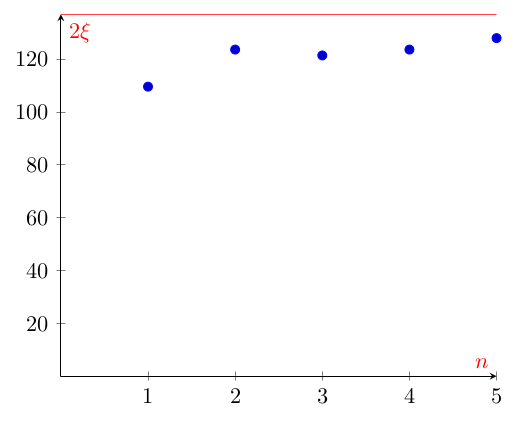
\includegraphics[width = 0.40\textwidth]{image/pic4.png}
    \caption{График зависимости $\xi (n)$}
\end{figure}

\subsection{Дифракция Фраунгофера на щели}

\begin{figure}[ht!]
    \centering
    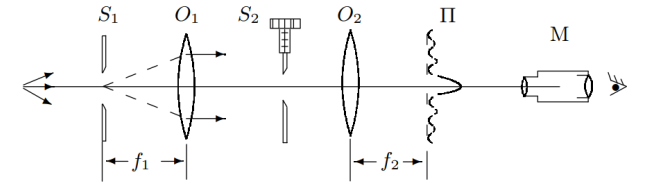
\includegraphics[width = 0.75\textwidth]{image/pic2.png}
    \caption{Схема лабораторной установки для наблюдения дифракции Фраунгофера на щели}
\end{figure}

\noindent Настроим установку, с помощью винта поперечного перемещения микроскопа измерим координаты
$X_m$ нескольких дифракционных минимумов от $-m$ до $m$. Занесём результаты в таблицу 2 (цена
деления шкалы ~0,02 мм).

\begin{table}[ht!]
    \centering
    \caption{Координаты минимумов дифракционной картины}
    \begin{tabular}{|c|c|c|c|c|c|c|c|c|c|}
    \hline
    $m$     & $-4$    & $-3$    & $-2$    & $-1$    & 0 & 1    & 2    & 3    & 4    \\ \hline
    дел.    & $-58$   & $-43$   & $-29$   & $-15$   & 0 & 15   & 29   & 43   & 58   \\ \hline
    $x$, мм & $-1,16$ & $-0,86$ & $-0,58$ & $-0,30$ & 0 & $0,30$ & $0,58$ & $0,86$ & $1,16$ \\ \hline
    \end{tabular}
    \end{table}

\begin{figure}[ht!]
    \centering
    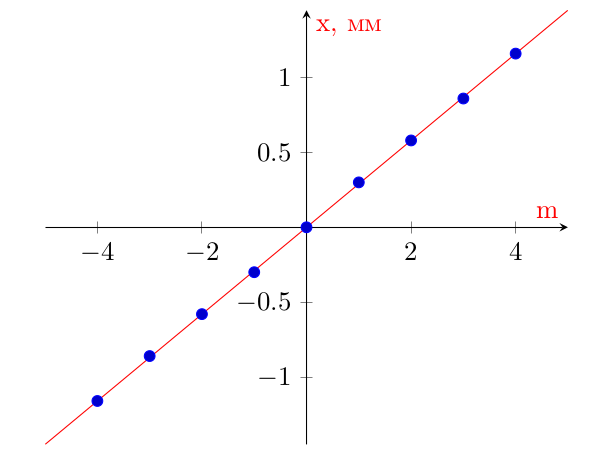
\includegraphics[width = 0.40\textwidth]{image/pic5.png}
    \caption{График зависимости $x(m)$}
\end{figure}

\subsection{Дифракция Фраунгофера на двух щелях}

В установке для дифракции Фраунгофера для одной щели заменяем щель $S_2$ экраном Э с двумя щелями. В итоге получаем характерное распределение максимумов и минимумов.

\noindent Определим расстояние между темными полосками внутри центрального максимума. Посчитаем число светлых промежутков между ними $$n = 6 \pm 1.$$ Измерим ширину центрального максимума $$X = 0,44 \pm 0,01 \;\; \text{мм}.$$ По полученным данным определим расстояние между минимумами $$\delta x = \frac{X}{n} = 73 \pm 10 \;\;\text{мкм}.$$ Откуда получим расстояние между щелями $$d = \frac{\lambda f_2}{\delta x} = 1,0 \pm 0,2 \;\;\text{мм}.$$

\subsection{Влияние дифракции на разрешающую способность оптического инструмента}

\begin{figure}[ht!]
    \centering
    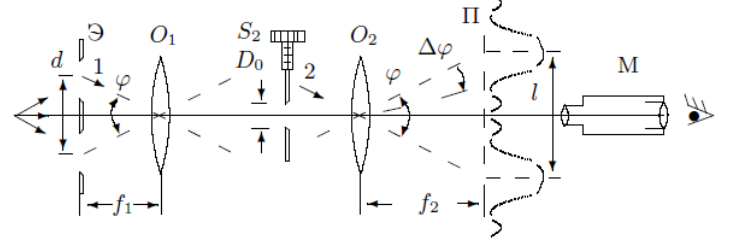
\includegraphics[width = 0.75\textwidth]{image/pic3.png}
    \caption{Исследование влияния дифракции на резрешающую способность оптического инструмента}
\end{figure}

\noindent Непосредственно из измерений получаем $$d_0 = 0,93 \pm 0,05 \;\; \text{мм},$$ $$D_1 = 0,18 \pm 0,01\;\; \text{мм},$$ $$D_2 = 0,36 \pm 0,01 \;\; \text{мм}.$$

\section{Вывод}

В ходе работы было изучено явление дифракции света --- дифракция Френеля на щели и на препятствии, дифракция Фраунгофера на одной и двух щелях.

\begin{itemize}
    \item При исследовании явления дифракции Френеля на щели убедились, что ширина зон Френеля примерно равна ширине щели

    \item При исследовании явления дифракции Фраунгофера на щели получили значение ширины щели, примерно равно измеренному непосредственно с помощью регулятора ширины щели:
    \begin{center}
        $b_0 = 223 $ мкм \hspace{1cm} $b_f = 242$ мкм
    \end{center}

    \item При исследовании явления дифракции Фраунгофера на двух щелях было получено значение расстояния между щелями, примерно равное измеренному с помощью микроскопа:
    
    \begin{center}
        $d_0 = 0,93$ мм \hspace{1cm} $d_f = 1$ мм
    \end{center}
\end{itemize}

\end{document}
